En el presente capítulo, se exploran las posibles mejoras y ajustes que pueden implementarse para lograr una representación más precisa y fidedigna del programa. Se abordan aspectos que permiten perfeccionar la integridad y la coherencia de la representación, buscando así optimizar el rendimiento y la comprensión del programa en cuestión.
\section{Cambios que se pueden realizar}
\begin{itemize}
    \item \textbf{Implementar mas funciones y equipamiento:} La principal premisa consistía en emplear los brazos robóticos sin necesidad de acudir al laboratorio ni contar con acceso directo al mismo. En consecuencia, se otorgó prioridad a la funcionalidad de dichos brazos, aunque esto ha implicado la carencia de equipo funcional dentro del laboratorio para lograr una simulación más precisa. Además, los brazos no poseen todas las funciones operativas.
    \item \textbf{Agregar una guía de uso:} Es viable desarrollar una guía interactiva que explique las funcionalidades básicas de los robots, con el objetivo de hacer la información más accesible y llegar a un público más amplio, especialmente a aquellos que no están familiarizados con el tema y desean aprender.
    \item \textbf{Mejorar modelos:} Uno de los cambios mas fundamentales que se debe realizar para mejorar la experiencia e intentar lograr ser lo mas fiel posible en la representación del laboratorio.
    Se puede empezar por realizar un modelado fiel y a escala real de los objetos presentes en el laboratorio, para esto se presenta el programa que provee Intelitek para su brazo Scorbot ER-4U.
    En la Figura \ref{fig:modelo} se presenta la interfaz del programa RoboCell, el cual sirve para darle instrucciones al brazo robótico, ya sea real o simulado, en este ultimo se ve el detallado del modelo que da mejor sensación de realismo.
\end{itemize}
\clearpage
\begin{figure}[h]
\centering
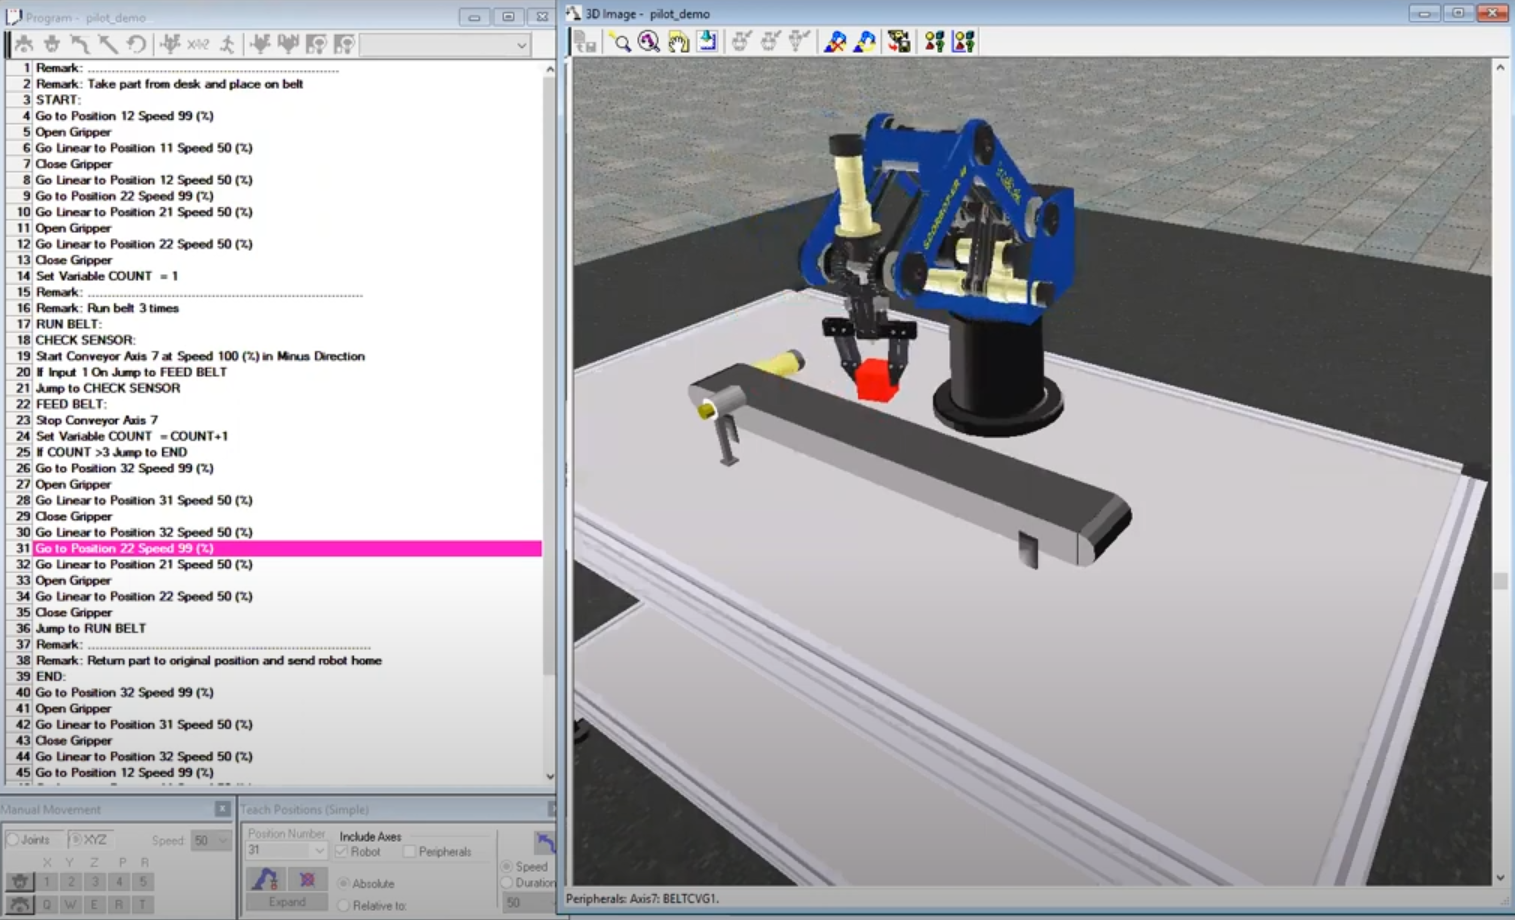
\includegraphics[width=13cm]{figures/modelo.png}
\caption{Diseño interfaz: Módulo Principal}
\label{fig:modelo}
\end{figure}
Estas son solo algunas ideas iniciales que pueden implementarse. La simulación no tiene límites, y el programa puede adaptarse para diversas finalidades, como la integración con la realidad virtual. Esto permitiría ampliar aún más las posibilidades de aprendizaje y entrenamiento, ofreciendo una experiencia inmersiva que podría abarcar desde el manejo básico de los brazos robóticos hasta aplicaciones más avanzadas en entornos simulados. Además, se podría explorar la opción de incorporar características de interactividad, permitiendo a los usuarios realizar prácticas y experimentos virtuales para consolidar sus conocimientos de manera práctica y segura. La flexibilidad del programa ofrece un amplio espectro de oportunidades para su expansión y adaptación a diferentes necesidades y contextos.